%!TEX root = Main.tex
\documentclass[Main]{subfiles}

\begin{document}

\section{Hardware} % (fold)
\label{sec:hardware}

	\subsection{Platform} % (fold)
	\label{sub:platform}

		The processing platform chosen for this project is a \emph{ZYBO Zynq\-7000 Development Board} from Digilent (see \autoref{fig:ZYBO}).
		The brains of the ZYBO is a Xilinx Zynq-7000 All Programmable System on a Chip (AP SoC).
		The AP SoC (see \autoref{fig:ZynqArch}) features both a Processing System (PS) consisting of a 650 MHz dual core ARM\textregistered{} Cortex A9 CPU with dedicated I/O, Memory and extensible FPGA Programmable Logic (PL) for HW synthesis.

		This enables the construction of a system with software, written in C++, running on the CPU, and with dedicated hardware for acceleration of computation and I/O handling.
		\begin{figure}[H]
			\centering
			\begin{subfigure}[b]{0.55\linewidth}
				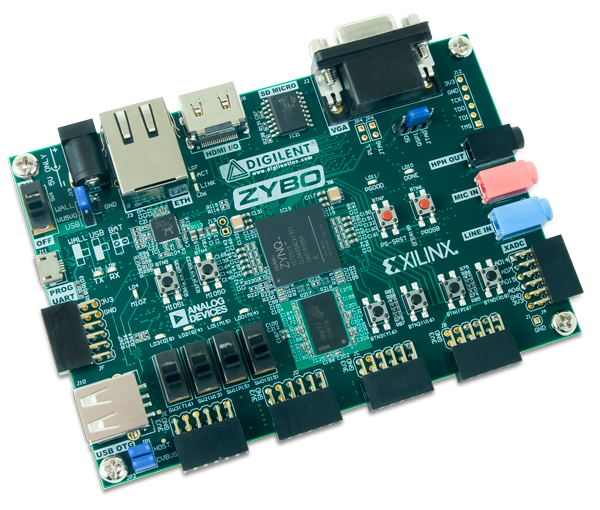
\includegraphics[width=\linewidth]{ZYBO}
				\caption{Digilent Zynq Board (ZYBO)}
				\label{fig:ZYBO}
			\end{subfigure}		
			\begin{subfigure}[b]{0.4\linewidth}
				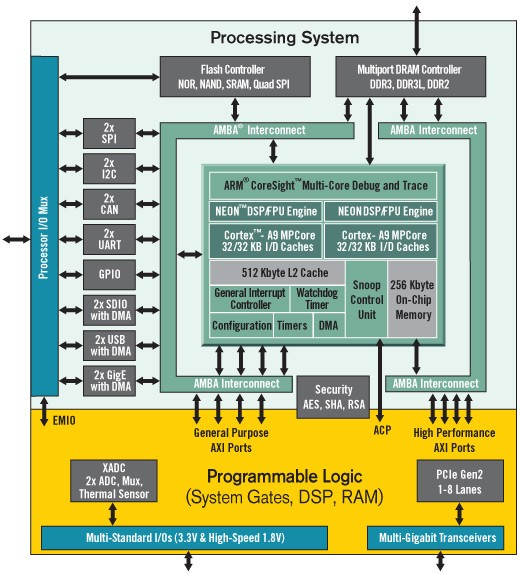
\includegraphics[width=\linewidth]{ZynqArch}
				\caption{Zynq-7000 AP SoC Diagram}
				\label{fig:ZynqArch}
			\end{subfigure}
			\caption{Figures borrowed from \cite{Digilent2014}}		
		\end{figure}

		Alongside the AP SoC the ZYBO features a range of external hardware for power supply/management and interfacing.
		It has push-buttons, throw-switches and LEDs for direct interface, USB-OTG, UART-to-USB and Ethernet for communication and HDMI, VGA and an audio codec for Audio/Visual.

		Lastly, the ZYBO features six PMOD GPIO ports along the perimeter (see \autoref{fig:ZYBO}), one directly connected to the PS and the others accessible through the PL.
		They deliver 3.3V power to external devices as well as eight customizable 1.8V or 3.3V digital I/O ports each (see \autoref{fig:pmod}).
		These are used for interfacing with the sensor and motor (see \autoref{sub:sensor} and \autoref{sub:motor_control}, respectively).

		\begin{figure}[H]
			\centering
			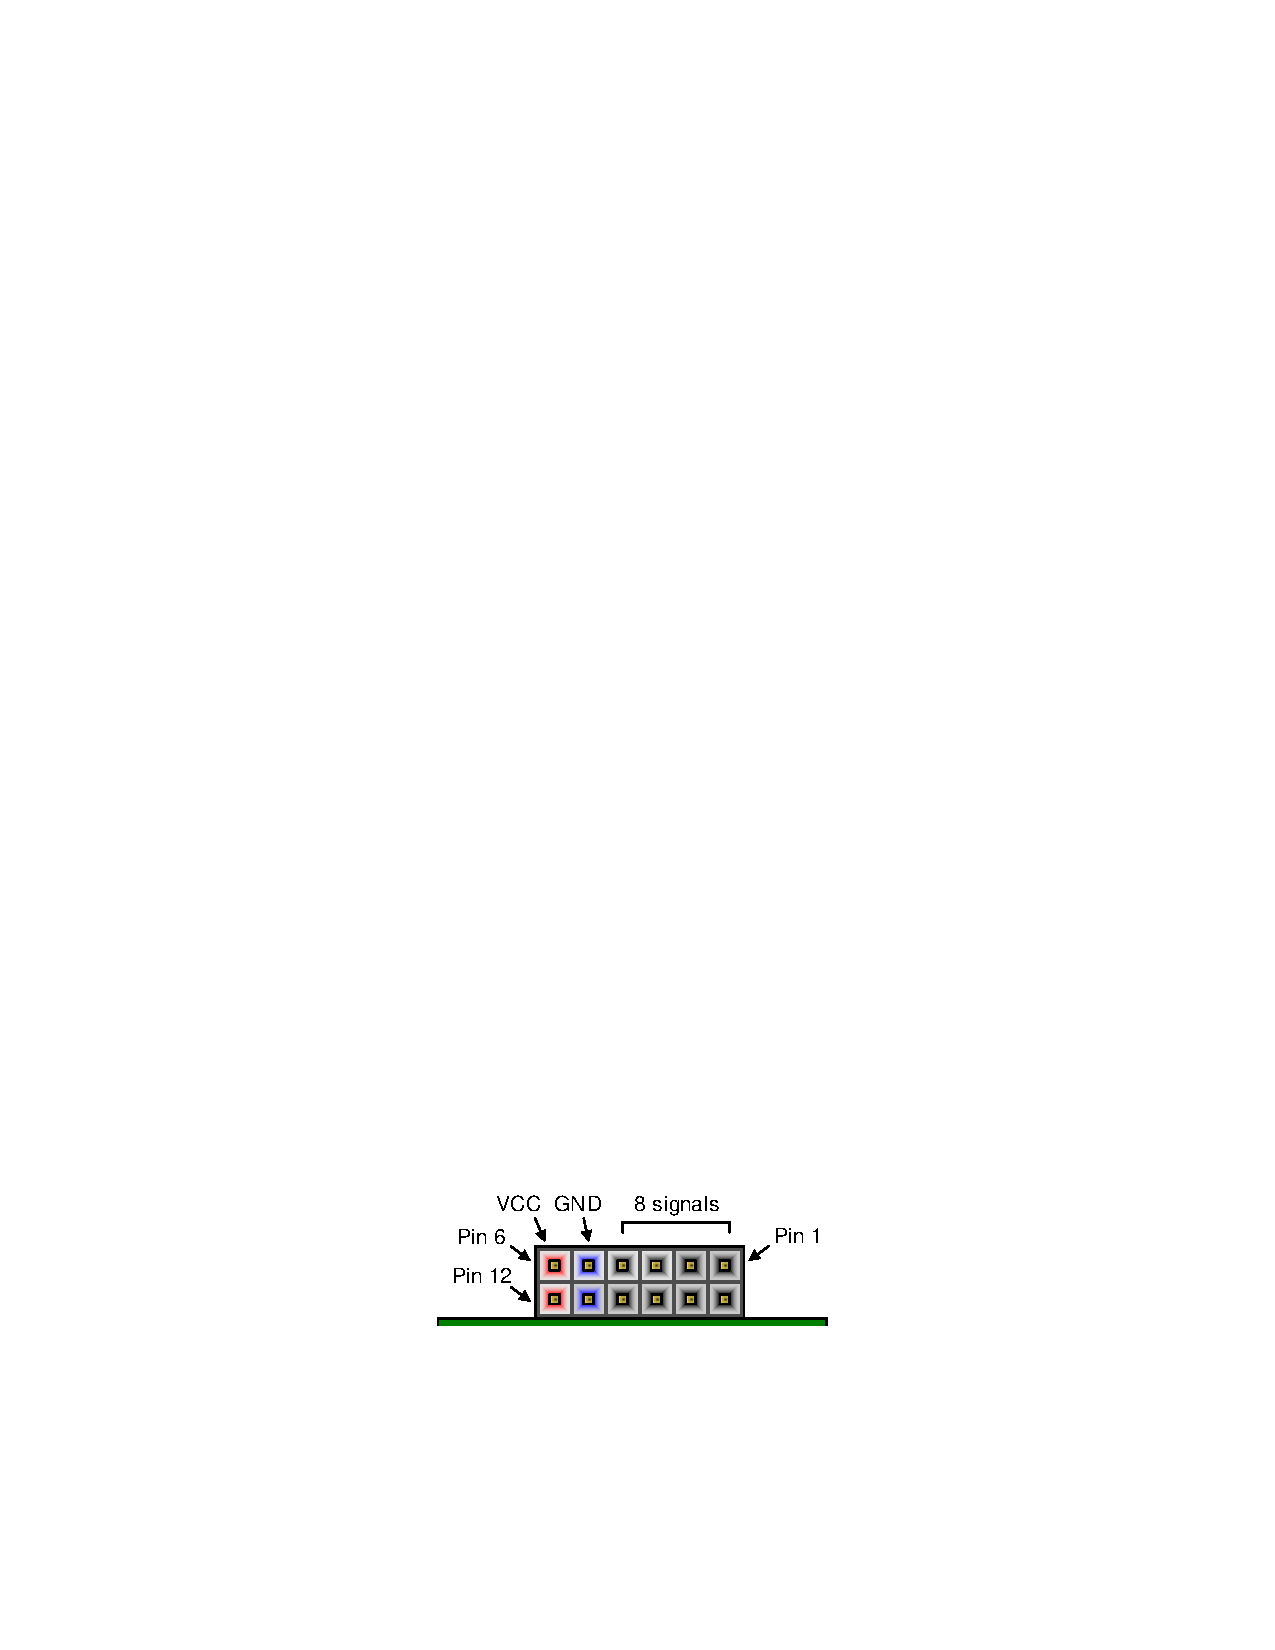
\includegraphics[width=0.5\linewidth]{PMOD_connector}
			\caption{PMOD Connector. Borrowed from \cite{Digilent2014}}
			\label{fig:pmod}
		\end{figure}

		\subsubsection{HW/SW Co-Design} % (fold)
		\label{ssub:hw_sw_co_design}

			The availability of FPGA logic on-chip enables rapid prototyping of HW acceleration blocks, through the use of High-Level Synthesis (HLS) tools.
			Using HLS one can specify some desired functionality in C++/SystemC code and directly synthesize it to HW-blocks to be implemented in FPGA logic, without needing to explicitly design HW in a Hardware Description Language like VHDL or Verilog.

			This is utilized for creating a PWM motor controller, described in \autoref{ssub:pwm_controller}.
			A desciption of the final design of the processing hardware include PS and designs in PL is found \autoref{sub:ap_soc_block_design}.
			
			% subsubsection hw_sw_co_design (end)
	
		% subsection platform (end)

	\subsection{Sensors} % (fold)
	\label{sub:sensor}

		The robot is designed to use a LIDAR (Light Detection and Ranging) sensor for sensing its location.
		The sensor chosen for this robot is a Neato XV-11 LDS (Laser Distance Sensor) (seen mounted atop the robot in \autoref{fig:final_robot}).
		This sensor consists of a 1 dimensional LDS mounted on a rotating platform, enabling it to take measurement in a 2 dimensional plane in 1\degree\ increments.
		The data is measured in mm at a numeric range of 0-16384 (14 bits) and an operating range of \textasciitilde 150-6000 mm depending on lighting conditions and reflectivity of objects.

		The top houses the sensor and computation unit. This measures the distance, measures rotational velocity of the sensor related to the base and handles communication of data.
		It requires a 3.3V power supply and consumes about 145 mA of current when operating and communicates via serial-communication (see \autoref{ssub:sensor_communication_protocol}).
		The top has four wires, connected via a slip ring. 
		The pinout is shown in \autoref{tab:lds_top}.

		The base houses the motor that drives the rotating top.
		The motor is designed to be powered by a pulse width modulated 12V power supply, but in this project the motor is power by a 3.3V continuous supply \.
		This consumes approximately 60 mA.

		\begin{table}[H]
			\begin{subtable}[b]{0.5\linewidth}
				\centering
					\begin{tabular}{|l|l|}
					\hline
					{\bf Wire} & {\bf Signal} \\ \hline
					Red        & +3.3V        \\ \hline
					Brown      & LDS\_RX      \\ \hline
					Orange     & LDS\_TX      \\ \hline
					Black      & GND          \\ \hline
				\end{tabular}
				\caption{LDS top pinout}
				\label{tab:lds_top}
			\end{subtable}
			\begin{subtable}[b]{0.5\linewidth}
				\centering
				\begin{tabular}{|l|l|}
					\hline
					{\bf Wire} & {\bf Signal} \\ \hline
					Red        & +3.3V        \\ \hline
					Black      & GND          \\ \hline
				\end{tabular}
				\caption{LDS motor pinout}
				\label{tab:lds_motor}
			\end{subtable}
			\caption{}
		\end{table}

		\newpage
		\subsubsection{Sensor data protocol} % (fold)
		\label{ssub:sensor_communication_protocol}
			The LDS transmits data via 3.3V RS-232 at 115200 BAUD.
			It uses 8 databits, no parity and one stop bit (\textbf{8N1}).
			Data is transmitted continuously while the sensor rotates, in packages of four readings, totaling in 90 packages per turn \cite{OpenSource}.

			Each package has 22 bytes in the following format:

			{\footnotesize\texttt{<start> <index> <speed\_L> <speed\_H> [Data 0] [Data 1] [Data 2] [Data 3] <checksum\_L> <checksum\_H>}}

			Where:
			\vspace{-12pt}
			\begin{itemize}
				\item \texttt{start} is always 0xFA

				\item \texttt{index} is the index byte in the 90 packets, going from 0xA0 (packet 0, readings 0 to 3) to 0xF9 (packet 89, readings 356 to 359)

				\item \texttt{speed} is a two-byte information, little-endian. It represents the speed, in 64th of RPM (aka value in RPM represented in fixed point, with 6 bits used for the decimal part)

				\item \texttt{[Data 0]} to \texttt{[Data 3]} are the 4 readings. Each one is 4 bytes long, and organized as follows 
				\begin{itemize}
					\item \texttt{<byte 0>} : \texttt{<distance 7:0>}

					\item \texttt{<byte 1>} : \texttt{<"invalid data" flag> <"strength warning" flag> <distance 13:8>}

					\item \texttt{<byte 2>} : \texttt{<signal strength 7:0>}

					\item \texttt{<byte 3>} : \texttt{<signal strength 15:8>}
				\end{itemize}
			\end{itemize}

			Data is only sensed and transmitted if the sensor is spinning at more than 180 PRM.
			If the sensor exceeds 320 RPM the data becomes sparse, as only every one in two measurements are non-zero and valid.
			Above 349 RPM the serial interface becomes a bottleneck and data is corrupted and packages are lost.

			Because we operate at near or above the 320 RPM limit we only the even numbered measurements are used.
			This way corruption will not occur with a varying amount of valid measurements being collected.

			% subsubsection sensor_communication_protocol (end)
	
		% subsection sensor (end)

	\subsection{Motor Control} % (fold)
	\label{sub:motor_control}

		The motor control hardware consists of two major blocks, an external Dual H-Bridge for driving the the motors, and an on-chip PWM controller for controlling the motor driver.
		The connection between the two blocks are shown in the SysML internal block diagram of the Motion block (\autoref{fig:motion_ibd}), along with the two motors.
		The \emph{Power}-signal comes from a battery (see \autoref{sub:power}), and \emph{Motor Control} is connected to the Processing System.

		\begin{figure}[H]
			\centering
			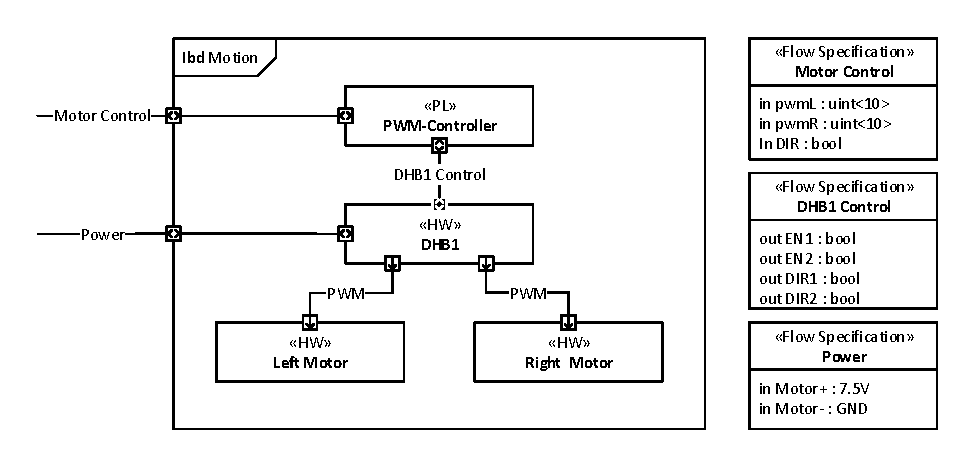
\includegraphics[width=1.0\linewidth]{MotionIBD}
			\caption{SysML Internal Block Diagram of the Motion Block}
			\label{fig:motion_ibd}
		\end{figure}

		\subsubsection{External Dual H-Bridge} % (fold)
		\label{ssub:external_dual_h_bridge}
			
			The \emph{DHB1} from Digilent is a dual- H-bridge motor controller that enables regular DC-motors to be driven in either direction with with a single ended power supply.
			Further it provides logic level transistor switching so that higher voltages (up to 11.8V) and higher currents (1.5A RMS, 2A peak) can be used to drive the motor without loading the logic circuit.

			\begin{figure}[H]
				\centering
				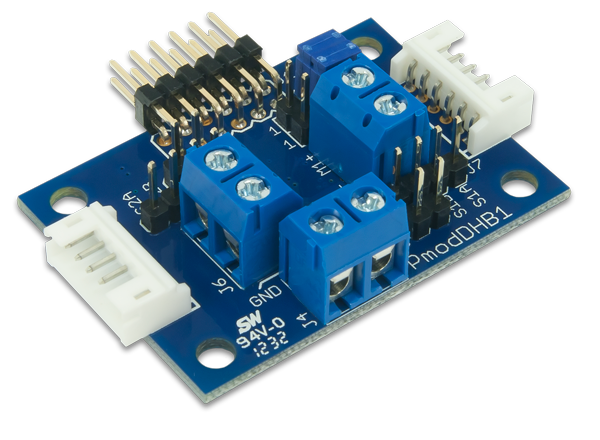
\includegraphics[width=0.6\linewidth]{PmodDHB1}
				\caption{Digilent PmodPHB1 Dual H-Bridge Motor controller \cite{Digilent2013}}
				\label{fig:DHB1}
			\end{figure}

			The DHB1 connects to the ZYBO via a PMOD connector. The individual signals are listed in \autoref{tab:dhb_pmod}.
			The motor power source is connected to the DHB1 with screw terminals. The two motors are also connected with screw terminals, but the left motor is connected with reversed polarity.
			This is because the identical motors need to spin in different directions to achieve the same rotation in relation to the direction of travel.

			\begin{table}[h]
				\centering
				\begin{subtable}[b]{0.6\linewidth}
					\begin{tabular}{|c|l|l|}
						\hline
						{\bf Pin} & {\bf Signal} & {\bf Description}         \\ \hline
						1         & EN1          & Motor 1 Enable            \\ \hline
						2         & DIR1         & Motor 1 Direction         \\ \hline
						3         & S1A          & Motor 1 Sensor A Feedback \\ \hline
						4         & S1B          & Motor 1 Sensor B Feedback \\ \hline
						5         & GND          & Power Supply Ground       \\ \hline
						6         & $V_{CC}$     & Power Supply (3.3V)       \\ \hline
						7         & EN2          & Motor 2 Enable            \\ \hline
						8         & DIR2         & Motor 2 Direction         \\ \hline
						9         & S2A          & Motor 2 Sensor A Feedback \\ \hline
						10        & S2B          & Motor 2 Sensor B Feedback \\ \hline
						11        & GND          & Power Supply Ground       \\ \hline
						12        & $V_{CC}$   & Power Supply (3.3V)       \\ \hline
					\end{tabular}
					\caption{PMOD connection description}
					\label{tab:dhb_pmod}
				\end{subtable}
				\begin{subtable}[b]{0.3\linewidth}
					\centering
					\begin{tabular}{ccl}
						\hline
						\multicolumn{1}{|c|}{{\bf DIR1}} & \multicolumn{1}{c|}{{\bf EN1}} & \multicolumn{1}{l|}{{\bf Result M1}} \\ \hline
						\multicolumn{1}{|c|}{0}          & \multicolumn{1}{c|}{0}         & \multicolumn{1}{l|}{Stop}            \\ \hline
						\multicolumn{1}{|c|}{0}          & \multicolumn{1}{c|}{1/PWM}     & \multicolumn{1}{l|}{Forward}         \\ \hline
						\multicolumn{1}{|c|}{1}          & \multicolumn{1}{c|}{0}         & \multicolumn{1}{l|}{Stop}            \\ \hline
						\multicolumn{1}{|c|}{1}          & \multicolumn{1}{c|}{1/PWM}     & \multicolumn{1}{l|}{Reverse}         \\ \hline
						                                 &                                &                                      \\ \hline
						\multicolumn{1}{|c|}{{\bf DIR2}} & \multicolumn{1}{c|}{{\bf EN2}} & \multicolumn{1}{l|}{{\bf Result M2}} \\ \hline
						\multicolumn{1}{|c|}{0}          & \multicolumn{1}{c|}{0}         & \multicolumn{1}{l|}{Stop}            \\ \hline
						\multicolumn{1}{|c|}{0}          & \multicolumn{1}{c|}{1/PWM}     & \multicolumn{1}{l|}{Forward}         \\ \hline
						\multicolumn{1}{|c|}{1}          & \multicolumn{1}{c|}{0}         & \multicolumn{1}{l|}{Stop}            \\ \hline
						\multicolumn{1}{|c|}{1}          & \multicolumn{1}{c|}{1/PWM}     & \multicolumn{1}{l|}{Reverse}         \\ \hline
					\end{tabular}
					\caption{Truth table for DHB-1 input}
					\label{tab:motor_signal}
				\end{subtable}
				\caption{} 
			\end{table} 

			To control the direction of the motor one applies a logic level to the \emph{DIR} pin for the corresponding motor; 1 for forward, 0 for reverse.
			The speed of the motors are controlled by applying a Pulse Width Modulated (PWM) signal to the EN pin for the corresponding motor (see \autoref{tab:motor_signal}).
			The sensor feedback pins are not used as there are no sensors attached to the wheels.

			For more information, see the reference manual \cite{Digilent2013}.

			% subsubsection external_dual_h_bridge (end)

		\subsubsection{PWM-controller} % (fold)
		\label{ssub:pwm_controller}
			
			The PWM-controller is implemented as a hardware IP-Core in the FPGA logic of the AP SoC.
			It has been modeled in SystemC code in the Vivado HLS tool.

			\autoref{lst:pwm_header} shows the header defining the PWM-controller module, consisting of a clock dividing thread and a PWM handling thread.
			It also defines the interface of \texttt{//Ports}, as designed in the IBD in \autoref{fig:motion_ibd}.

			\newpage
			\lstinputlisting[caption=PWM-Controller SystemC Header, style=Code-C++, label=lst:pwm_header, basicstyle=\scriptsize]{../MotorControl/MotorControl/main.h}

			\newpage
			\lstinputlisting[caption=PWM-Controller SystemC Definition, style=Code-C++, label=lst:pwm_definition, basicstyle=\scriptsize]{../MotorControl/MotorControl/main.cpp}

			\autoref{lst:pwm_definition} shows the definition of the module declared in \autoref{lst:pwm_header}.
			The \texttt{clockDividerThread} is responsible for dividing the 100 MHz clock of the PL down to a 2 MHz clock that can be used for ticks in the \texttt{pwmThread}.
			The use of a 2 MHz PWM-clock is based on the choice of a 10 bit resolution and a recommendation from \cite{Digilent2013} of a ~2 kHz PWM-cycle for the DHB1.

			\begin{equation}
				f_{PWMclock}
				\frac{f_{PL}}{ONE\_TICK} =
				\frac{100\ \text{MHz}}{25} =
				2\ \text{MHz}
			\end{equation}

			\begin{equation}
				f_{PWMcycle} =
				\frac{f_{PWMclock}}{2^{PWM\ resolution}} =
				\frac{2\ \text{MHz}}{2^{10}} =
				\frac{2\ \text{MHz}}{1024} =
				1.953\ \text{kHz}
				\approx 2\ \text{kHz}
			\end{equation}

			\texttt{clockDividerThread} signals \texttt{pwmThread} of a PWM clock tick by setting \texttt{pwmClock} for one PL clock-cycle every time a PWM clock tick is generated.

			\texttt{pwmThread} handles PWM output by counting up a 10 bit variable everytime it receives a PWM clock tick, and compares the count with the PWM settings for the left and right motor, \texttt{pwmL} and \texttt{pwmR} respectively.
			If the count is below the PWM setting, the enable signal is held high, and if it is above it is held low.
			This way the output duty cycle is determined by:
			\begin{equation}
				DC = \frac{PWM\ setting}{1024}
				\quad \quad \text{Example: }
				\frac{512}{1024} = 50\%
			\end{equation}

			This model was then synthesized to VHDL code using the Vivado HLS tool and imported into the overall block design.
			Using special \texttt{\#pragma}'s the setting variables \texttt{pwmL}, \texttt{pwmR} and \texttt{DIR} are mapped onto the AXI memory bus of the AP SoC.
			This way they are readily addressable from the PS as memory mapped registers.
			The procedure for controlling the motors from software is described in \autoref{subsub:software_robotframe}.


			% subsubsection pwm_controller (end)
		
		% subsection motor_control (end)

	\subsection{AP SoC Block Design} % (fold)
	\label{sub:ap_soc_block_design}

		\autoref{fig:zybocar_design} shows the final block design for the AP SoC designed in \emph{Vivado}.
		In the top left corner the Processing system is shown and below it is a reset controller. 
		In the middle is the memory mapped AXI Interconnect Bus.

		In the top right \emph{MotorCtrl} is the PWM controller, described in \autoref{ssub:pwm_controller}.
		Below \emph{MotorCtrl} is \emph{AXI GPIO}; a GPIO controller used to interface with the push-buttons on the ZYBO.
		Lastly, in the bottom right corner, \emph{AXI Uartlite} is a UART synthesized in PL.
		This is used to interface the LDS sensor with the PS via the AXI Interconnect bus.

		\begin{figure}[H]
			\centering
			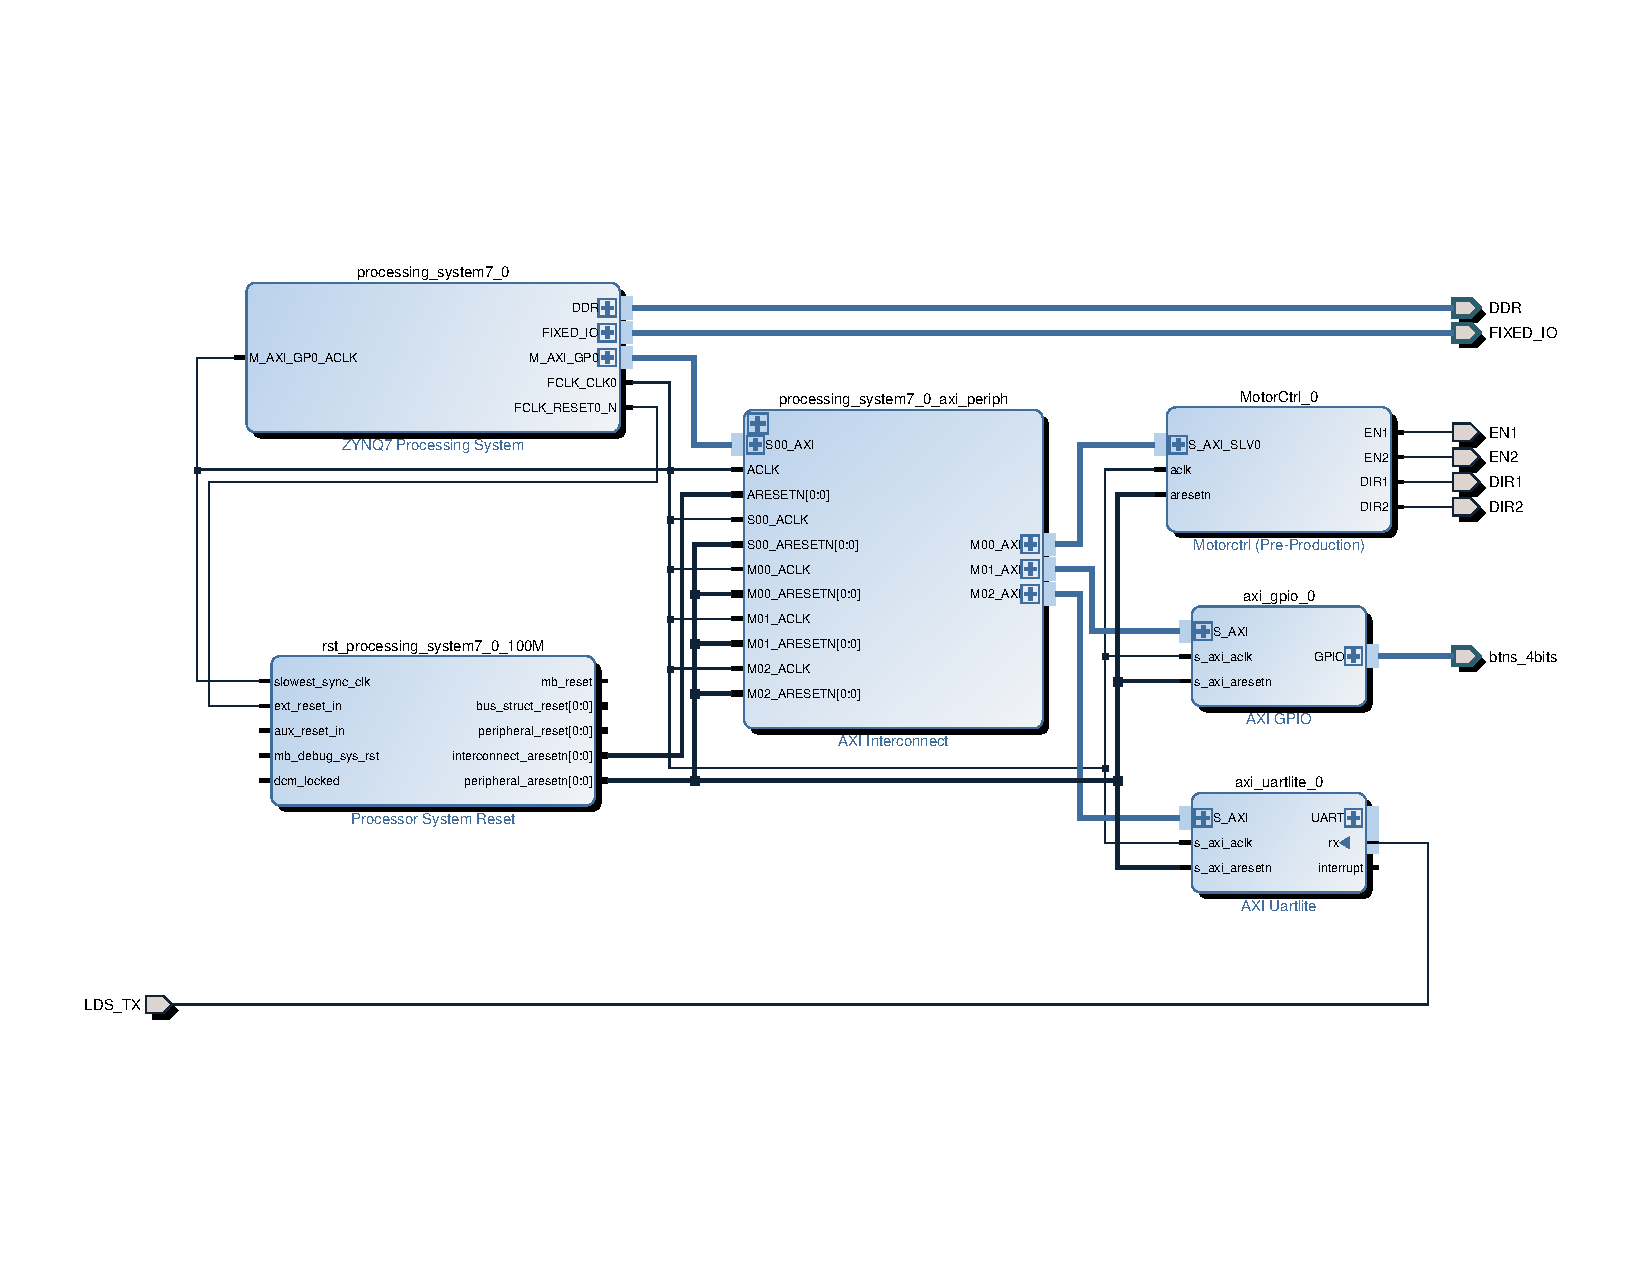
\includegraphics[width=\linewidth]{ZyboCarDesign}
			\caption{ZyboCar Hardware Platform Block Design}
			\label{fig:zybocar_design}
		\end{figure}
		This block design is synthesized and a \emph{hardware wrapper}, along with a \emph{bitstream} for programming a device, is generated and exported for use with the \emph{Xilinx SDK} IDE.
		The SDK is then used for writing the \emph{bitstream} to the ZYBO and programming the PS. 

		% subsection ap_soc_block_design (end)

	\subsection{Power} % (fold)
	\label{sub:power}

		This project uses three different power sources: 7.5V, 5V and 3.3V.
		The 7.5V supply comes from a battery bank of 5 1.5V AA batteries\fxnote{Picture}.
		This is used solely for powering the motors, and is connected to the DHB1.
		The 5V supply comes from a micro-USB power bank. \fxnote{picture}
		It is used to power the ZYBO.

		The 3.3V supply is supplied by the ZYBO's on-board power regulator.
		The ZYBO can supply a theoretical maximum of 2.5A (minus its own consumption $\sim150\ to\ 400\ mA$) with a maximum of 1A supplied to each PMOD.
		The output is however limited by the output of the 5V power bank.
		Assuming little to no conversion loss the the maximum current from the ZYBO 3.3V supply is:
		\begin{equation}
			P_{PB} = I_{PB} * V_{PB} = 
			500\ mA * 5\ V =
			2.5\ W
		\end{equation}
		\begin{equation}
			I_{3V3} = 
			\frac{P_{PB}}{3.3\ V} =
			757.57\ mA
		\end{equation}
		The 3.3V supply is used to power the LDS top and motor through one PMOD connector and the DHB1 through another.

		% subsection power (end)

	% section hardware (end)

\end{document}
